%--------------------------------------------------------------------------------------------------------------------------------
% DON'T ADD OR REMOVE ANY PACKAGES
\documentclass{article}
\usepackage{graphicx}
\usepackage{float}
\usepackage{url} % Required for the Bibliography Reference Url
\usepackage{hyperref}
%--------------------------------------------------------------------------------------------------------------------------------

%--------------------------------------------------------------------------------------------------------------------------------
% TODO: Set title, author and date
\title{Exploring Fractal Art in Complex Numbers}
\author{23bXXXX}
\date{April, 2024}
%--------------------------------------------------------------------------------------------------------------------------------

\begin{document}

% TODO: Apply the title
\maketitle
%--------------------------------------------------------------------------------------------------------------------------------
% TODO: Create a section "Introduction"
\section{Introduction}
% Write the line here, it should look like:-
% ""Look at this simple quadratic recurrence equation:""
Look at this simple quadratic recurrence equation:
% TODO: Write the equation using \begin{equation}. See the equation in expected_main.pdf file.
% Make a label for it as well.
\begin{equation}
    z_{n+1} = z_{n}^{2} + c
    \label{eq:eqn}
\end{equation}
% Write the line here, it should look like:-
% ""Where""
Where
% TODO: Create those 2 bullet points. See expected_main.pdf to see how they look like.
\begin{itemize}
    \item $z$ is a complex number
    \item $c$ is a constant
\end{itemize}
% Write the line here, it should look like:-
% ""We will see now how this seemingly simple equation can produce amazingly beautiful patterns in the complex plane.""
We will see now how this seemingly simple equation can produce amazingly beautiful patterns in the complex plane.
%--------------------------------------------------------------------------------------------------------------------------------

%--------------------------------------------------------------------------------------------------------------------------------
% TODO: Create a section "Fractal Art Gallery"
\section{Fractal Art Gallery}
% TODO: Create the table.
\begin{table}[htbp]
  \centering
  \begin{tabular}{|c|c|}
    \hline
    \textbf{Artwork} & \textbf{Artist} \\
    \hline
    Mandelbrot Madness & John Smith \\
    Cosmic Chaos & Emily Johnson \\
    Fractal Symphony & David Williams \\
    \hline
  \end{tabular}
\end{table}
% TODO: Write the line here, it should look like:-
% ""These artists explore the fascinating world of fractal art by manipulating complex numbers to create stunning visual representations of mathematical concepts. For more info, see %%%%%3%%%%%.""
% Replace %%%%%3%%%%% with a citation to the reference as mentioned in Problem Statement.
These artists explore the fascinating world of fractal art by manipulating complex numbers to create stunning visual representations of mathematical concepts. For more info, see \cite{link}.
%--------------------------------------------------------------------------------------------------------------------------------

%--------------------------------------------------------------------------------------------------------------------------------
% TODO: Create a section "Mandelbrot Set"
\section{Mandelbrot Set}
% TODO: Create a subsection "Definition"
\subsection{Definition}
% TODO: Write the line here, it should look like:-
% ""The Mandelbrot set is the set of all c for which Equation %%%%%1%%%%%, starting from $z = 0$, does not diverge to %%%%%2%%%%%.""
% %%%%%1%%%%%  and  %%%%%2%%%%% are same as for Julia Set section.
The Mandelbrot set is the set of all c for which Equation \ref{eq:eqn}, starting from $z = 0$, does not diverge to $\infty$.
% TODO: Create a subsection "Definition"
\subsection{Diagram}
% TODO: Insert the image mandelbrot.png using \begin{figure}[H]. Set width as half of \textwidth. Put the needed caption.
\begin{figure}[H]
  \centering
  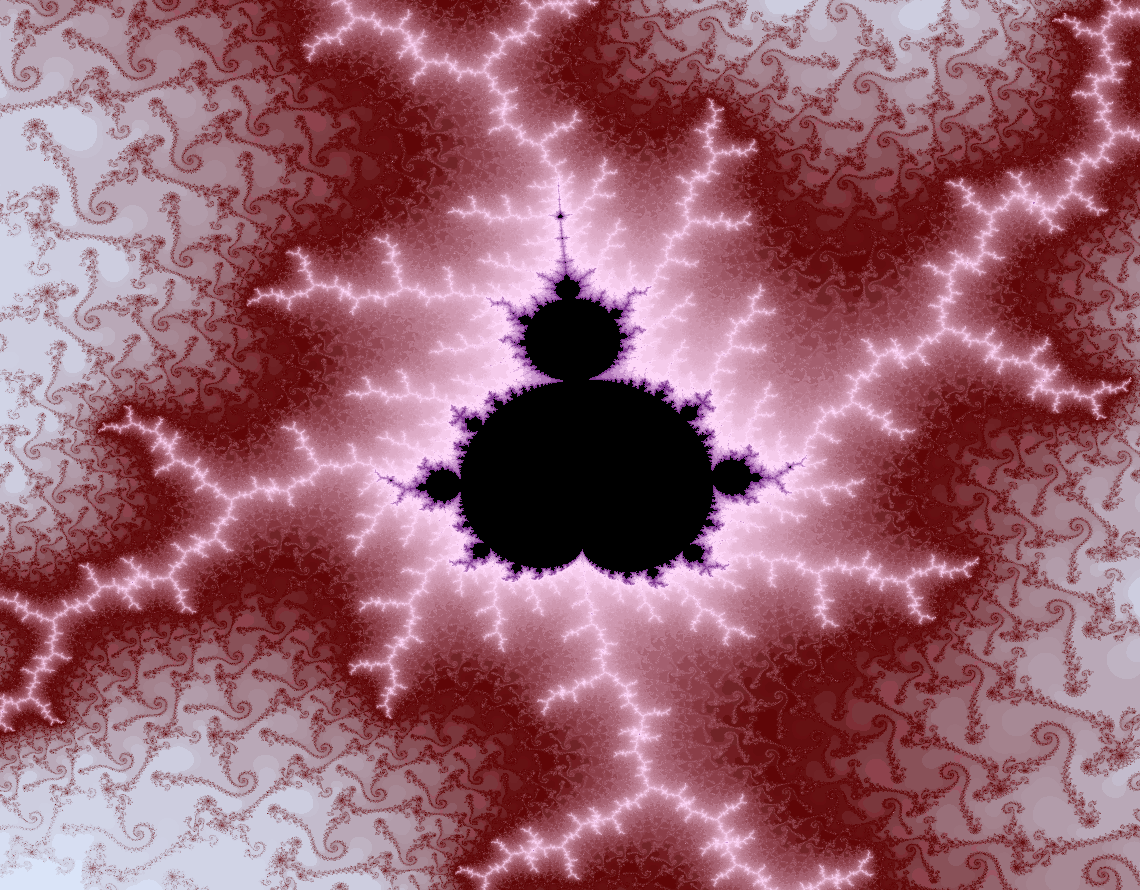
\includegraphics[width=0.5\textwidth]{mandelbrot.png}
  \caption{The Mandelbrot Set}
\end{figure}
%--------------------------------------------------------------------------------------------------------------------------------

%--------------------------------------------------------------------------------------------------------------------------------
% Insert commands to deal with bibtex
\bibliographystyle{plain}
\bibliography{references}
%--------------------------------------------------------------------------------------------------------------------------------

\end{document}
